\documentclass[11pt]{article}

% ── Core layout ───────────────────────────────────────────────────────────────
\usepackage[top=1in, bottom=1in, left=1.15in, right=1.15in]{geometry}
\usepackage{microtype}
\usepackage{lmodern}
\usepackage[T1]{fontenc}
\usepackage[utf8]{inputenc}

% ── Fonts ─────────────────────────────────────────────────────────────────────
\usepackage{palatino}          % Body font: Palatino (reads like a report, not a paper)
\usepackage{helvet}            % Section font: Helvetica

% ── Color ─────────────────────────────────────────────────────────────────────
\usepackage[dvipsnames,svgnames,table]{xcolor}
\definecolor{NavyReport}{RGB}{15,  40,  80}   % Deep navy  – headers
\definecolor{AccentBlue}{RGB}{0,   90, 160}   % Mid blue   – rules / highlights
\definecolor{LightGray} {RGB}{245,245,245}    % Near-white – table row shading
\definecolor{MidGray}   {RGB}{180,180,180}    % Rule gray

% ── Section styling ───────────────────────────────────────────────────────────
\usepackage{titlesec}
% Section: navy, sans-serif, left rule accent
\titleformat{\section}
  {\color{NavyReport}\fontfamily{phv}\fontseries{b}\fontsize{13}{15}\selectfont}
  {}{0em}
  {\colorbox{NavyReport}{\parbox{4pt}{\strut}}\hspace{6pt}}
\titlespacing*{\section}{0pt}{18pt}{6pt}

% Subsection: accent blue, sans-serif
\titleformat{\subsection}
  {\color{AccentBlue}\fontfamily{phv}\fontseries{b}\fontsize{11}{13}\selectfont}
  {}{0em}{}
\titlespacing*{\subsection}{0pt}{12pt}{4pt}

% Subsubsection: small-caps, dark
\titleformat{\subsubsection}[runin]
  {\fontfamily{phv}\fontseries{b}\fontsize{10}{12}\selectfont\color{NavyReport}}
  {}{0em}{}
\titlespacing*{\subsubsection}{0pt}{8pt}{6pt}

% ── Header / Footer ───────────────────────────────────────────────────────────
\usepackage{fancyhdr}
\pagestyle{fancy}
\fancyhf{}
\fancyhead[L]{\fontfamily{phv}\fontsize{8}{10}\selectfont\color{MidGray}%
  Credit Approval Rule Analysis}
\fancyhead[R]{\fontfamily{phv}\fontsize{8}{10}\selectfont\color{MidGray}%
  MIT Sloan $\cdot$ 15.C51 $\cdot$ Spring 2026}
\fancyfoot[C]{\fontfamily{phv}\fontsize{8}{10}\selectfont\color{MidGray}\thepage}
\renewcommand{\headrulewidth}{0.4pt}
\renewcommand{\headrule}{\color{MidGray}\hrule width\headwidth height\headrulewidth}

% ── Tables ────────────────────────────────────────────────────────────────────
\usepackage{booktabs}
\usepackage{array}
\usepackage{tabularx}
\usepackage{float}
\usepackage{caption}
\captionsetup{
  font={small, sf},
  labelfont={bf, color=NavyReport},
  labelsep=period,
  skip=4pt
}
% Alternating row shading helper
\usepackage{colortbl}
\newcommand{\rowhead}{\rowcolor{NavyReport!15}}
\newcommand{\rowalt}{\rowcolor{LightGray}}

% ── Figures ───────────────────────────────────────────────────────────────────
\usepackage{graphicx}

% ── Lists ─────────────────────────────────────────────────────────────────────
\usepackage{enumitem}
\setlist[itemize]{leftmargin=1.4em, itemsep=1pt, topsep=3pt}
\setlist[enumerate]{leftmargin=1.4em, itemsep=1pt, topsep=3pt}

% ── Paragraph spacing ─────────────────────────────────────────────────────────
\usepackage{parskip}
\setlength{\parskip}{5pt}
\setlength{\parindent}{0pt}

% ── Hyperlinks ────────────────────────────────────────────────────────────────
\usepackage[hidelinks]{hyperref}
\hypersetup{
  colorlinks=true,
  linkcolor=AccentBlue,
  citecolor=AccentBlue,
  urlcolor=AccentBlue
}

% ── Bibliography ──────────────────────────────────────────────────────────────
\usepackage[numbers]{natbib}

% ── Misc ──────────────────────────────────────────────────────────────────────
\usepackage{setspace}
\usepackage{amsmath}

% ══════════════════════════════════════════════════════════════════════════════
%  COVER PAGE
% ══════════════════════════════════════════════════════════════════════════════
\newcommand{\coverpage}{%
  \thispagestyle{empty}
  % Top navy bar
  {\color{NavyReport}\rule{\linewidth}{6pt}}\\[2pt]
  {\color{AccentBlue}\rule{\linewidth}{1.5pt}}
  \vspace{2.4cm}

  % Report type label
  {\fontfamily{phv}\fontseries{b}\fontsize{9}{11}\selectfont
   \color{AccentBlue}\MakeUppercase{Analytical Report}}

  \vspace{0.5cm}

  % Title
  {\fontfamily{phv}\fontseries{b}\fontsize{26}{30}\selectfont
   \color{NavyReport} Credit Approval Rule Analysis}\\[0.5em]
  {\fontfamily{phv}\fontseries{m}\fontsize{14}{17}\selectfont
   \color{AccentBlue} Explainability-First Machine Learning Pipeline}

  \vspace{0.6cm}
  {\color{MidGray}\rule{\linewidth}{0.6pt}}
  \vspace{0.4cm}

  % Subtitle / dataset
  {\fontfamily{phv}\fontsize{10}{12}\selectfont
   \color{NavyReport}
   UCI Credit Approval Dataset $\cdot$ Random Forest $\cdot$ SHAP Explainability}

  \vfill

  % Bottom metadata block
  {\color{MidGray}\rule{\linewidth}{0.6pt}}\\[8pt]
  \begin{minipage}[t]{0.55\linewidth}
    {\fontfamily{phv}\fontseries{b}\fontsize{9}{11}\selectfont\color{NavyReport}
     Submitted to}\\[3pt]
    {\fontfamily{phv}\fontsize{9}{12}\selectfont\color{NavyReport}
     Prof.\ Andrew W.\ Lo \&\ Prof.\ Paul F.\ Mende\\[1pt]
     15.C51 $\cdot$ Modeling with Machine Learning: Financial Technology\\[1pt]
     MIT Sloan School of Management}
  \end{minipage}%
  \hfill
  \begin{minipage}[t]{0.35\linewidth}
    \raggedleft
    {\fontfamily{phv}\fontseries{b}\fontsize{9}{11}\selectfont\color{NavyReport}
     Date}\\[3pt]
    {\fontfamily{phv}\fontsize{9}{12}\selectfont\color{NavyReport} Spring 2026}
  \end{minipage}
  \\[6pt]
  {\color{NavyReport}\rule{\linewidth}{3pt}}
  \newpage
}

% ══════════════════════════════════════════════════════════════════════════════
\begin{document}
\coverpage

% TOC
{\hypersetup{linkcolor=NavyReport}
\tableofcontents}
\newpage

% ──────────────────────────────────────────────────────────────────────────────
\section{Executive Summary}
% ──────────────────────────────────────────────────────────────────────────────

This report examines the UCI Credit Approval dataset using an explainability-first machine learning pipeline. The objective is not to build a production-ready credit scoring system. It is to use a stable, well-validated model as an analytical instrument for understanding which features drive credit approval decisions, how those features interact, and what the results imply for fairness and regulatory compliance in algorithmic lending.

The dataset contains 690 observations across 15 fully anonymized features and one binary outcome. After removing 37 incomplete observations, 653 clean cases remain. The class distribution is 45.3\% approved and 54.7\% denied. A Random Forest classifier, selected under a stability-first criterion across 10-fold stratified cross-validation, achieves a mean AUC of 0.9366 with a standard deviation of 0.0282 (Table~\ref{tab:model}).

The central findings are as follows. A9 is the dominant predictor, with a mean absolute SHAP value of 0.2034~---~three times the next highest feature. Its effect is binary and directionally stable across 8 of 10 cross-validation folds. A10, A11, and A8 form a correlated secondary cluster: their SHAP contributions are real but substantially shared with A9. A15 and A14 carry independent information, though A15's positive effect is concentrated in the extreme upper tail of its distribution and A14's effect is direction-unstable. Table~\ref{tab:importance} summarizes the full feature importance picture. Protected characteristics A1 and A7 contribute near-zero SHAP values and do not drive model decisions.

The fair lending analysis identifies two concerns independent of model intent. A15's tail effect raises disparate impact questions if the feature proxies wealth or income. Feature anonymization creates a compliance barrier that would prevent deployment under the Equal Credit Opportunity Act, the Fair Credit Reporting Act, and the EU AI Act's high-risk AI provisions, which classify credit scoring systems as high-risk from August 2026 (Table~\ref{tab:regulatory}).

% ──────────────────────────────────────────────────────────────────────────────
\section{Context and Scope}
% ──────────────────────────────────────────────────────────────────────────────

\subsection{Credit Approval as a Decision Problem}

Credit approval decisions sit at the intersection of financial risk management and consumer access to capital. A lender's core objective is to distinguish applicants who will repay from those who will not, using observable information available at the time of application. Traditional approaches rely on structured scorecards derived from logistic regression, where the contribution of each variable is explicit and the decision boundary is interpretable by design \citep{khandani2010}. Machine learning models offer greater predictive flexibility, particularly in the presence of nonlinear relationships and feature interactions, but introduce a tradeoff between accuracy and interpretability that has direct regulatory implications.

The literature on machine learning in consumer credit is substantial. \citet{khandani2010} demonstrate that nonlinear ML models applied to transaction-level data produce meaningful improvements in delinquency prediction over traditional scorecards. \citet{butaru2016} analyze credit card risk across six major US banks and find that risk factors differ significantly across institutions, suggesting that no single model structure generalizes cleanly across lending portfolios. Both studies underscore a recurring theme: predictive performance and model transparency are not automatically aligned, and the institutional context shapes which tradeoff is acceptable.

\subsection{The Dataset and Its Constraints}

This analysis uses the UCI Credit Approval dataset, a real-world collection of consumer credit applications from an unidentified financial institution. The dataset was contributed to the UCI Machine Learning Repository with all feature names and values deliberately anonymized to protect applicant confidentiality \citep{quinlan1987}. The outcome variable indicates binary approval or denial. The institutional context, geographic origin, time period, and credit product type are unknown. Table~\ref{tab:dataset} summarizes the key dataset properties.

The anonymization is a defining constraint of this analysis. Any interpretive claim about what the model has learned is conditional on assumptions about what the features represent, and those assumptions cannot be verified. This constraint is revisited in each section of the report where it bears on the conclusions drawn.

\subsection{Scope and Objective}

This report does not aim to build a production-ready credit scoring system. The dataset is too small, the features are anonymous, and the institutional context is unknown. The objective is narrower: to use a stable, well-validated machine learning model as an analytical instrument for understanding what patterns drive credit approval decisions in this dataset, and what those patterns imply for fairness, auditability, and the broader deployment of algorithmic decision systems in lending.

The question of how AI interacts with credit ecosystems is not primarily a question about model accuracy. It is a question about which features carry predictive signal, whether that signal is stable across data partitions, whether it is consistent with the principles of fair lending, and whether the decision process it encodes can be explained to the applicants it affects and the regulators who oversee it. This analysis addresses each of these questions in turn, within the limits imposed by the data.

% ──────────────────────────────────────────────────────────────────────────────
\section{Key Findings}
% ──────────────────────────────────────────────────────────────────────────────

\subsection{Feature Importance and the Role of A9}

A9 is the dominant predictor in this dataset by a substantial margin. Its mean absolute SHAP value across the full analytical sample is 0.2034. The next highest feature, A11, registers 0.0682. No other feature exceeds 0.07. Table~\ref{tab:importance} provides the full feature importance summary across all metrics. Because the model was selected for stability rather than peak accuracy, as described in Section~\ref{sec:model}, these importance rankings reflect consistent signal rather than artifacts of a single favorable data split.

\begin{table}[H]
\centering
\caption{Feature importance summary.}
\label{tab:importance}
\setlength{\arrayrulewidth}{0.4pt}
\begin{tabular}{lccccl}
\toprule
\rowhead
\color{white}\textbf{Feature} &
\color{white}\textbf{SHAP Rank} &
\color{white}\textbf{Mean $|$SHAP$|$} &
\color{white}\textbf{Perm.\ Importance} &
\color{white}\textbf{Corr.\ with A9} &
\color{white}\textbf{Fold Stability} \\
\midrule
A9  & 1 & 0.2034 & High     & ---  & 8/10 \\
\rowalt
A11 & 2 & 0.0682 & Moderate & 0.38 & 2/10$^\dagger$ \\
A8  & 3 & 0.0559 & Moderate & 0.34 & 5/10 \\
\rowalt
A15 & 4 & 0.0454 & High     & 0.06 & 3/10$^\dagger$ \\
A10 & 5 & 0.0419 & Moderate & 0.43 & 8/10 \\
\rowalt
A14 & 6 & 0.0255 & Moderate & 0.08 & 4/10 \\
A6  & 7 & 0.0220 & Low      & ---  & 4/10 \\
\rowalt
A3  & 8 & 0.0199 & Low      & ---  & 3/10 \\
\bottomrule
\multicolumn{6}{l}{\footnotesize $^\dagger$ Fold stability reflects skewed distribution artifact; beeswarm on full model is the correct directional diagnostic.}\\
\multicolumn{6}{l}{\footnotesize See Sections~\ref{sec:cluster} and~\ref{sec:limitations}.}
\end{tabular}
\end{table}

The structure of A9's effect is binary rather than continuous. The SHAP beeswarm plot (Figure~\ref{fig:beeswarm}) shows two distinct clusters. Low values of A9 produce large negative SHAP contributions, pushing predicted approval probability downward. High values produce large positive contributions, pushing it upward. There is no gradual middle range. Applicants with low A9 values face a strong prior against approval that the remaining features cannot easily overcome.

This directional effect is stable across data partitions. A9 produces a positive fold-mean SHAP value in 8 of 10 cross-validation folds (Figure~\ref{fig:signmatrix}). The two dissenting folds reflect sampling variation. The bimodal structure visible in the beeswarm is consistent across all folds individually.

\begin{figure}[H]
\centering
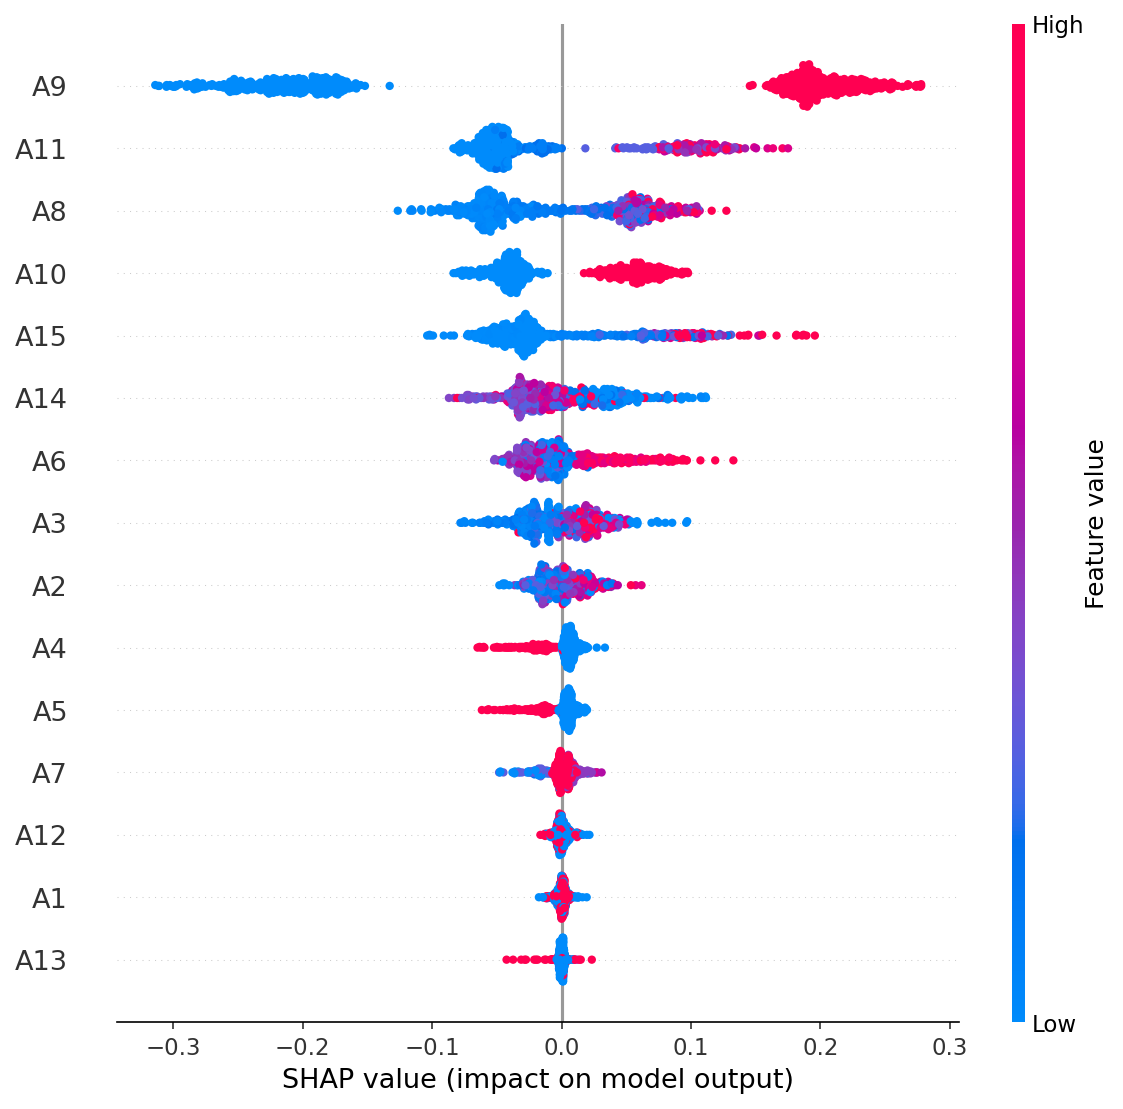
\includegraphics[width=0.80\linewidth]{figures/fig1_beeswarm.png}
\caption{SHAP beeswarm plot for the final model trained on all 653 observations. Features are sorted by mean $|$SHAP$|$ (descending). Color encodes raw feature value (red~=~high, blue~=~low). Horizontal position encodes effect on approval probability.}
\label{fig:beeswarm}
\end{figure}

\subsection{Correlated Features: A10, A11, and A8}
\label{sec:cluster}

A10, A11, and A8 occupy the top tier of SHAP magnitude after A9 and rank second through fourth in permutation importance (Figure~\ref{fig:permutation}). All three are positively correlated with A9: Pearson correlations of 0.43, 0.38, and 0.34 respectively (Figure~\ref{fig:correlation}). The distinction between permutation importance and SHAP importance is relevant here. High permutation importance indicates independent predictive contribution when all other features are present. High SHAP magnitude with relatively lower permutation importance indicates that a feature's contribution is partially shared with correlated features. A10, A11, and A8 exhibit the latter pattern. Their SHAP contributions are real, but a substantial portion of that signal overlaps with A9.

A11 and A8 share a similar response shape. Both show a rapid positive increase at low feature values that saturates quickly, consistent with a log-shaped threshold effect (Figure~\ref{fig:pdpice}, PDP panel). The ICE curves fan widely for both features, indicating that the marginal effect of each varies substantially across individual applicants. A10 follows a binary structure closer to A9, producing either a clearly positive or clearly negative SHAP contribution with little in between.

The fold-level sign stability matrix (Figure~\ref{fig:signmatrix}) shows A10 at 8/10 positive folds, consistent with its beeswarm profile. A11 registers only 2/10 positive folds. For features with highly left-skewed distributions, the fold-level mean SHAP is dominated by the large mass of near-zero observations, pulling the mean negative even when the feature produces positive contributions for elevated-value applicants. The beeswarm on the full model is the more reliable diagnostic for A11's directional effect. This limitation is discussed in Section~\ref{sec:skew}.

\begin{figure}[H]
\centering
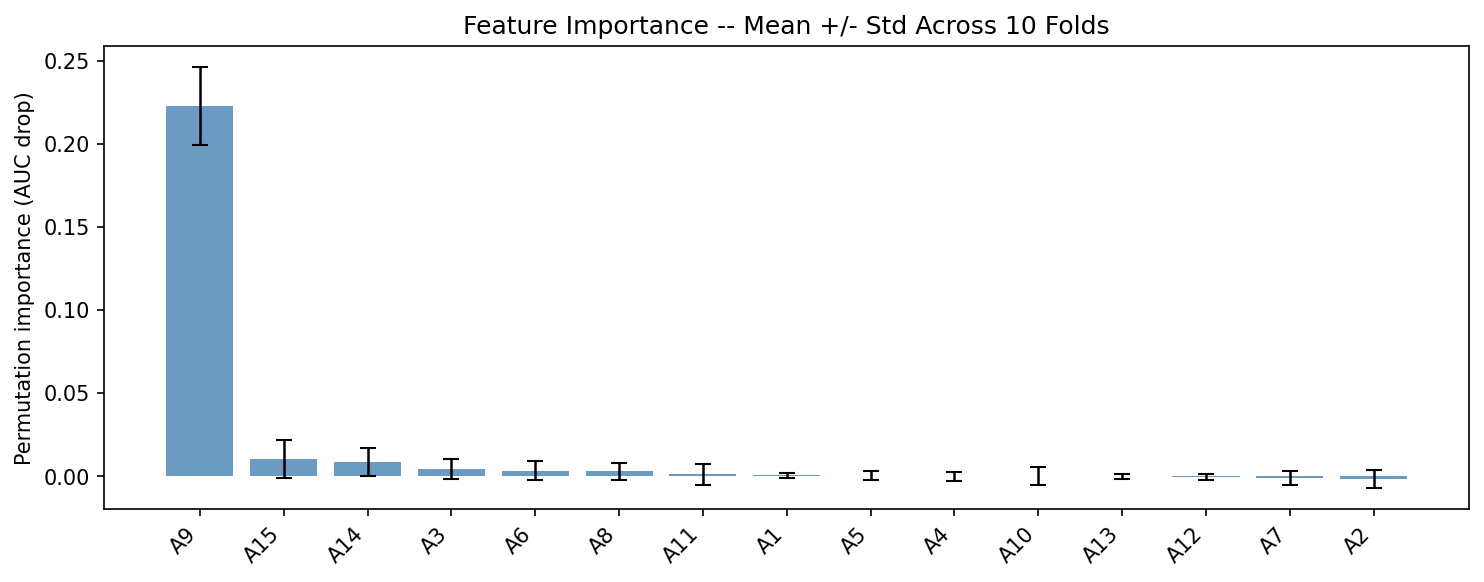
\includegraphics[width=0.85\linewidth]{figures/fig2_permutation.png}
\caption{Permutation feature importance~--- mean $\pm$ std across 10 cross-validation folds. Error bars represent one standard deviation.}
\label{fig:permutation}
\end{figure}

\begin{figure}[H]
\centering
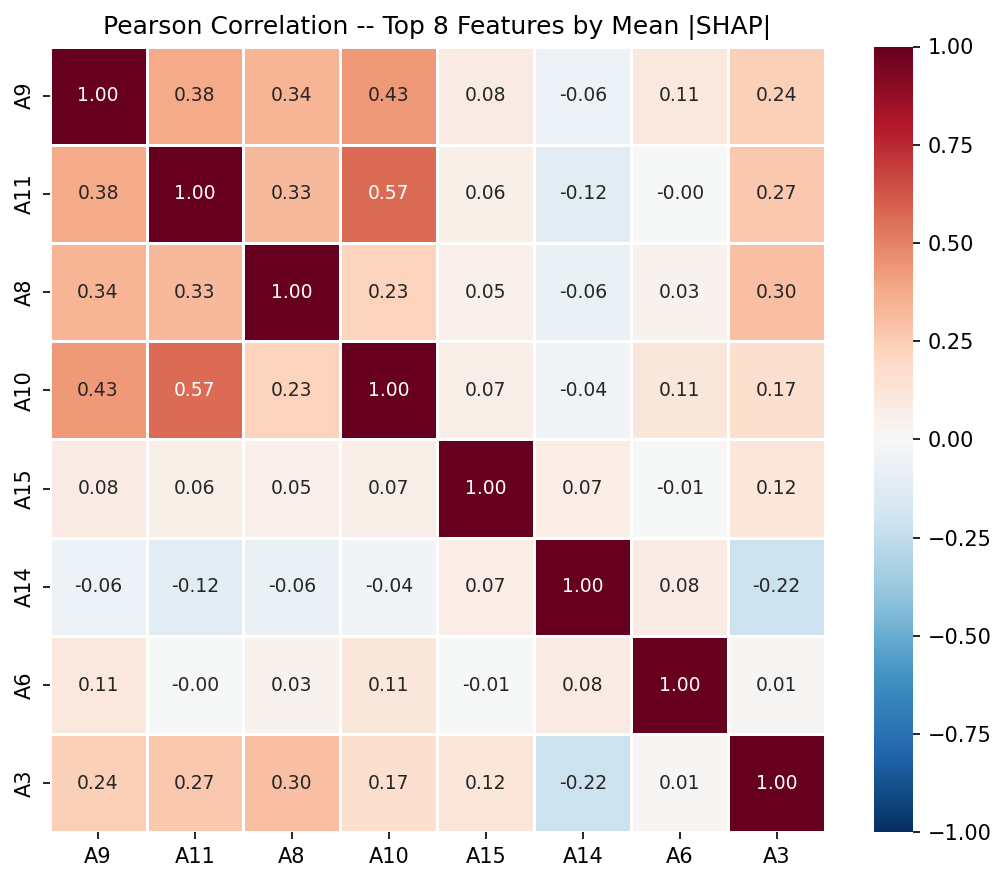
\includegraphics[width=0.65\linewidth]{figures/fig3_correlation.png}
\caption{Pearson correlation heatmap among the top 8 features ranked by mean $|$SHAP$|$. Warm red~=~positive correlation; cool blue~=~negative.}
\label{fig:correlation}
\end{figure}

\subsection{Orthogonal Signals: A15 and A14}

A15 and A14 are not part of the A9 correlated cluster. Their correlations with A9 are 0.06 and 0.08 respectively (Figure~\ref{fig:correlation}). They carry information that is independent of the primary signal and its associated features.

A15 produces near-zero SHAP values for most applicants. For a small subset at the extreme upper tail of the A15 distribution, it generates a meaningfully positive contribution to predicted approval probability (Figures~\ref{fig:beeswarm} and~\ref{fig:pdpice}). Below that threshold, A15 is effectively inert. The fold-level sign matrix places A15 at 3/10 positive folds, again reflecting the skew limitation described in Section~\ref{sec:cluster}. The beeswarm and PDP both confirm the tail-positive structure independently.

A14 is the weakest feature among the top signals. Its PDP is nearly flat across its full range (Figure~\ref{fig:pdpice}), and its ICE curves cross heavily, indicating that the marginal effect reverses direction across individuals. The fold-level sign matrix places A14 at 4/10 positive folds. No stable directional interpretation for A14 is consistent across the diagnostics used in this analysis.

\begin{figure}[H]
\centering
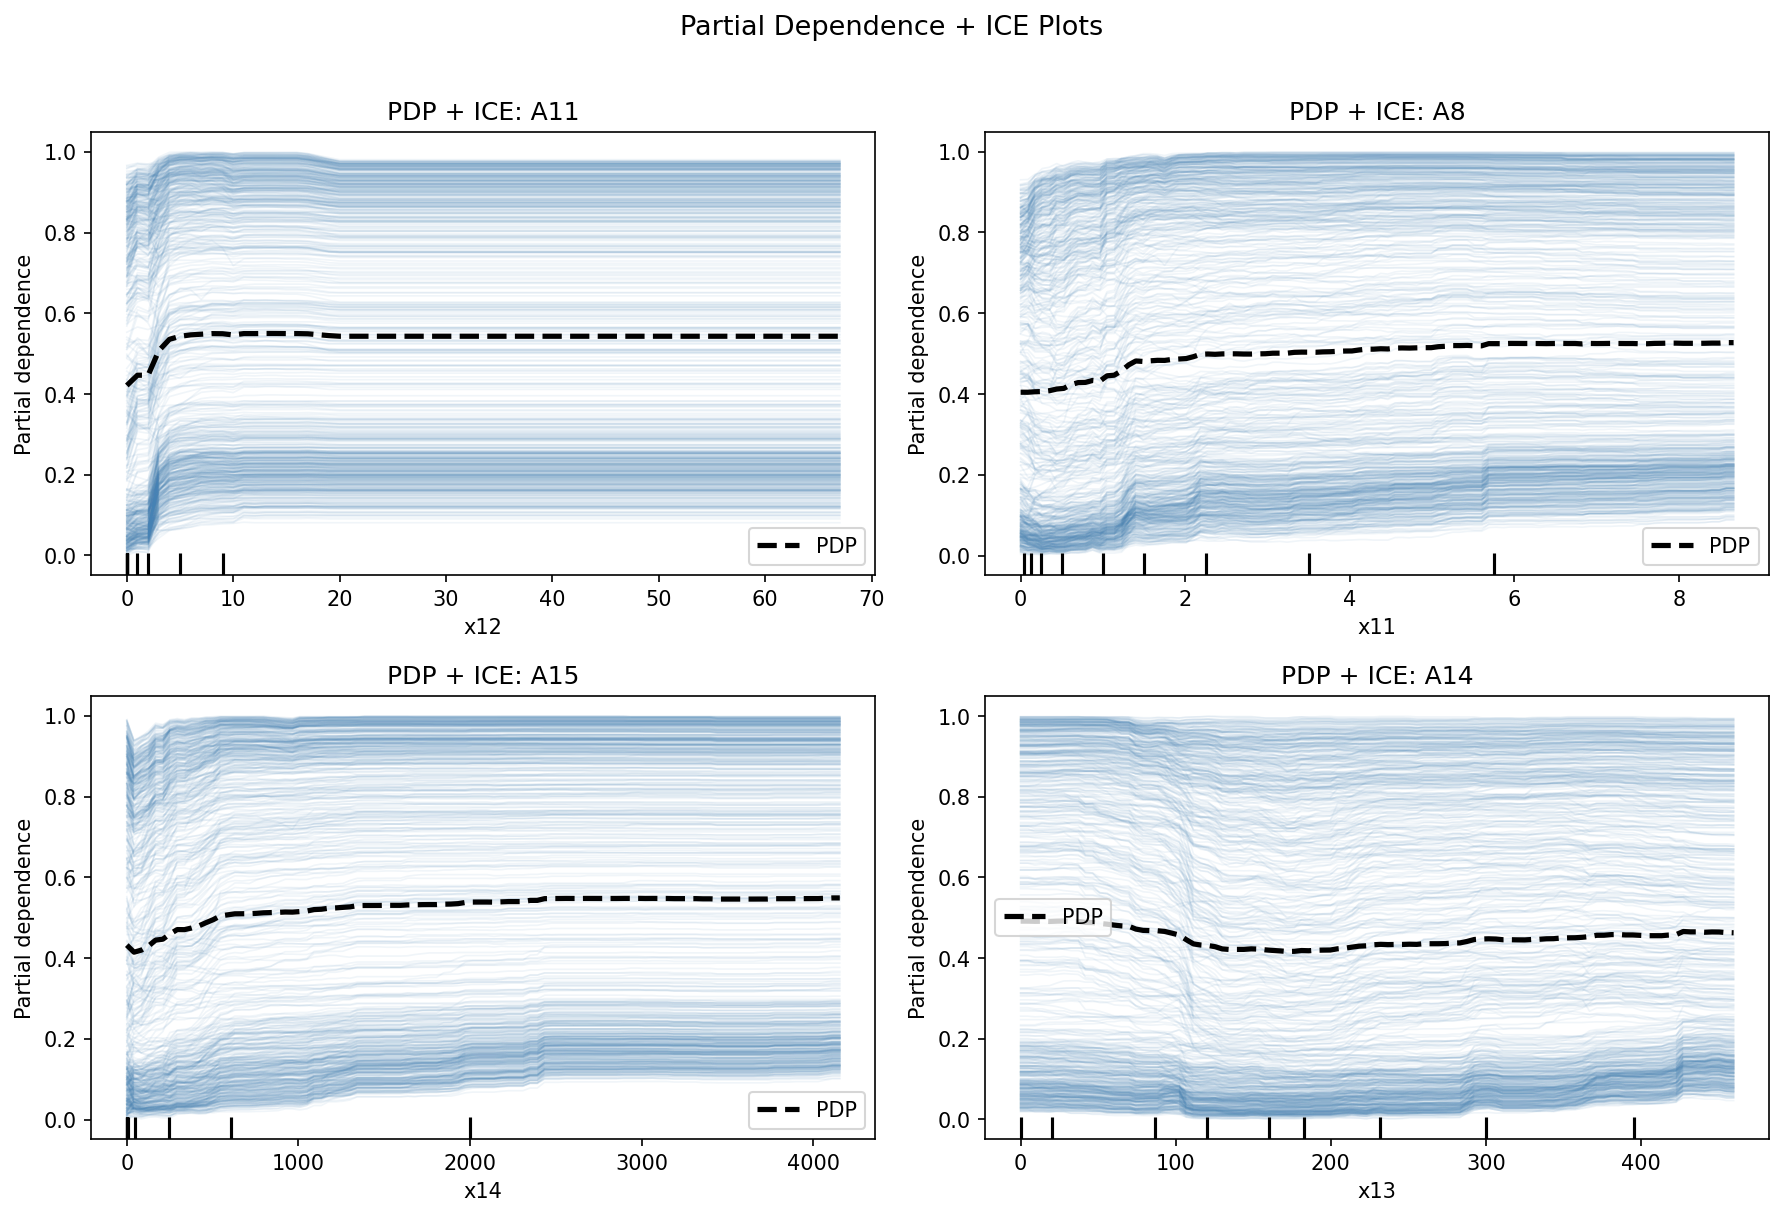
\includegraphics[width=\linewidth]{figures/fig4_pdp_ice.png}
\caption{PDP~+~ICE plots for A11, A8, A15, and A14. The dashed line shows the population-average partial dependence. Thin lines show individual conditional expectations for a random subsample of 200 observations.}
\label{fig:pdpice}
\end{figure}

\subsection{Low-Importance and Direction-Unstable Features}

The remaining features~--- A3, A5, A6, A2, A1, A4, A7, A12, and A13~--- contribute near-zero SHAP values in the full model and show no consistent directional pattern in the sign stability matrix (Figure~\ref{fig:signmatrix}). A5 and A8 are the most directionally unstable, each splitting evenly across positive and negative fold means. A3 and A6 show a weak negative lean at 3/10 and 4/10 positive folds respectively, but their SHAP magnitudes are too small to support reliable conclusions.

A1 and A7 warrant separate note. Based on the structure of the UCI Credit Approval dataset and prior literature on credit application features, A1 is commonly interpreted as a binary sex or gender indicator, and A7 as an indicator related to ethnicity or national origin. Both are protected characteristics under major fair lending frameworks. Both rank at the bottom of the SHAP importance ranking and contribute effectively zero to model predictions. This is addressed in Section~\ref{sec:fairlending}.

\begin{figure}[H]
\centering
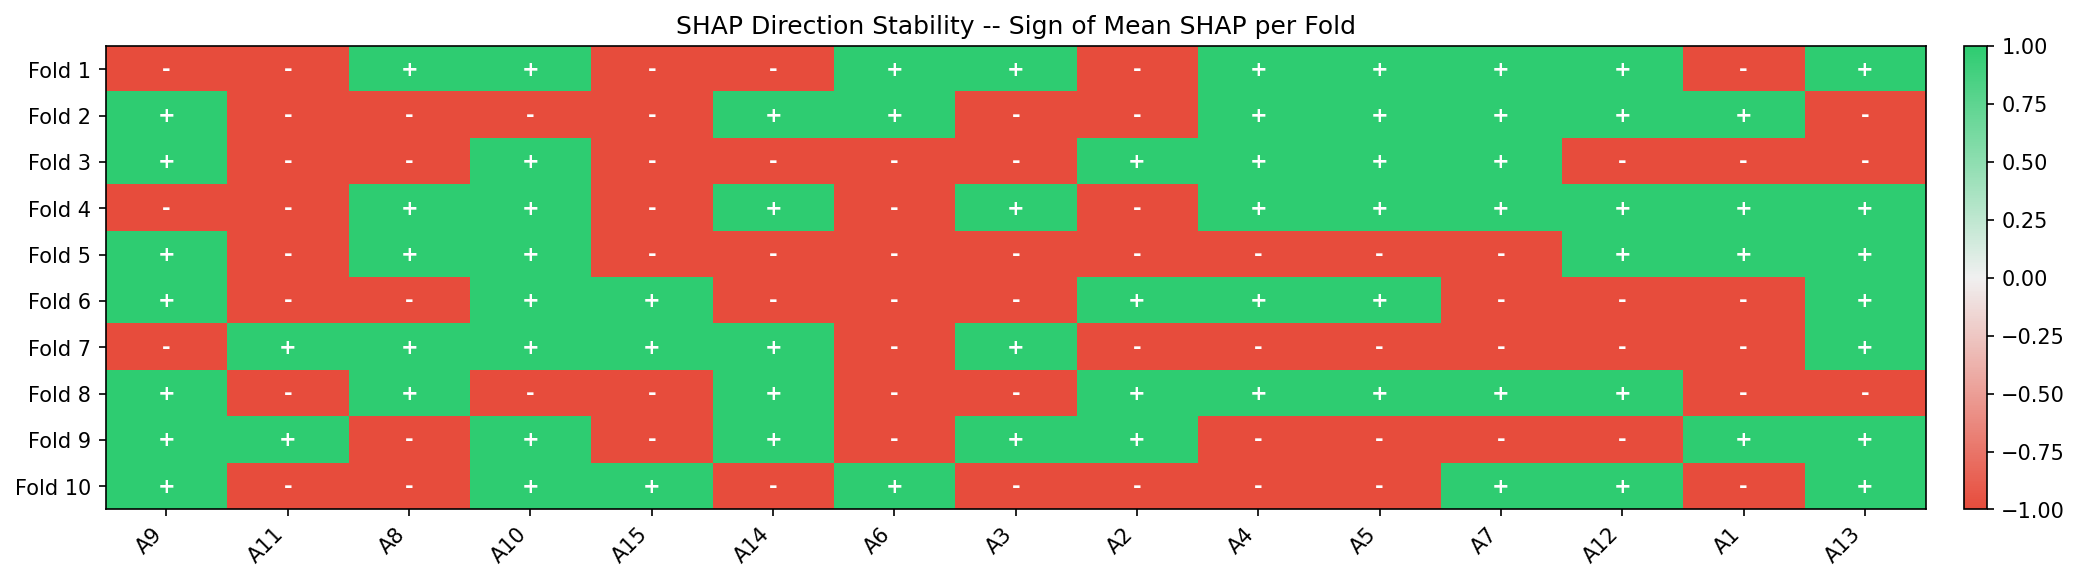
\includegraphics[width=\linewidth]{figures/fig5_sign_matrix.png}
\caption{SHAP direction stability matrix. Each cell shows the sign of the mean SHAP value for that feature in that fold: `+' (green) pushes toward approval; `-' (red) pushes toward denial.}
\label{fig:signmatrix}
\end{figure}

\subsection{Fair Lending Analysis}
\label{sec:fairlending}

\subsubsection*{Disparate treatment}

Disparate treatment occurs when a model uses protected characteristics as direct inputs to reach differential outcomes. Under the Equal Credit Opportunity Act (ECOA) and Regulation~B, creditors are prohibited from discriminating on the basis of race, color, religion, national origin, sex, marital status, or age \citep{cfpb2022}. In this model, A1 and A7 are present as features but contribute near-zero SHAP values. The model does not materially rely on these characteristics to reach approval decisions. This is a positive finding from a disparate treatment standpoint. It does not, however, exhaust the fair lending analysis.

\subsubsection*{Disparate impact}

Disparate impact concerns arise when a facially neutral feature produces outcomes that disproportionately disadvantage a protected class. A15's tail effect is the primary candidate for this concern. The feature is effectively inert for most applicants and provides a meaningful approval boost only for those at the extreme upper end of its distribution. If A15 proxies wealth, income, or accumulated assets, the structural effect is to selectively reward applicants with exceptional financial resources. In most credit markets, access to exceptional financial resources correlates with race, national origin, and other protected characteristics due to historical and structural factors. This does not make A15 an impermissible feature, but any deployment of a model with this structure would require a formal disparate impact analysis and, where adverse impact is found, a documented search for less discriminatory alternatives \citep{dobbie2024, asurity2024}.

\subsubsection*{Compliance barrier under feature anonymization}

A lending institution cannot deploy a model built on anonymous features in any major jurisdiction. Under ECOA and Regulation~B, creditors must provide applicants with specific reasons for adverse action decisions. \citet{cfpb2022} explicitly addresses this requirement in the context of complex machine learning models, affirming that the use of algorithmic models does not exempt creditors from the obligation to provide specific and accurate adverse action notices. A model whose features cannot be identified or described in human-readable terms cannot satisfy this requirement.

\subsubsection*{Regulatory exposure across jurisdictions}

Regulatory constraints on algorithmic credit scoring extend beyond the United States. Table~\ref{tab:regulatory} summarizes the compliance status of a model of this type across the three most relevant regulatory frameworks.

\begin{table}[H]
\centering
\caption{Regulatory exposure by jurisdiction.}
\label{tab:regulatory}
\setlength{\arrayrulewidth}{0.4pt}
\begin{tabularx}{\textwidth}{llXl}
\toprule
\rowhead
\color{white}\textbf{Jurisdiction} &
\color{white}\textbf{Framework} &
\color{white}\textbf{Key Requirement} &
\color{white}\textbf{Status} \\
\midrule
United States & ECOA / Regulation B & Specific adverse action reasons required & Non-compliant \\
\rowalt
United States & FCRA & Accurate disclosure of factors affecting credit decisions & Non-compliant \\
European Union & EU AI Act, Annex III \S5(b) & Risk management, technical documentation, human oversight, EU database registration (from Aug 2026) & Non-compliant \\
\bottomrule
\end{tabularx}
\end{table}

This points to a broader structural problem in the deployment of algorithmic credit systems. As these systems become more capable and more widely adopted, the gap between what a model can predict and what a regulator can audit is widening. \citet{kozodoi2022} provide a framework for formally testing and optimizing fairness in credit scoring models, demonstrating that accuracy and fairness are not necessarily in tension and that the tradeoff between them can be explicitly managed. \citet{dumitrescu2022} benchmark twelve bias mitigation methods across multiple credit datasets, finding substantial variation in outcomes across methods and datasets. Both bodies of work reach the same conclusion: fair lending compliance in algorithmic systems requires proactive formal analysis. Without feature identity, that analysis cannot begin.

% ──────────────────────────────────────────────────────────────────────────────
\section{Data and Methodology}
\label{sec:model}
% ──────────────────────────────────────────────────────────────────────────────

\subsection{Data}

This analysis uses the UCI Credit Approval dataset, a publicly available benchmark comprising 690 observations of consumer credit applications with a binary outcome variable \citep{quinlan1987}. The dataset contains 15 anonymized predictor features~--- nine categorical and six continuous~--- with all feature names and values deliberately obscured to protect applicant confidentiality. Table~\ref{tab:dataset} summarizes the key dataset properties.

\begin{table}[H]
\centering
\caption{Dataset summary.}
\label{tab:dataset}
\setlength{\arrayrulewidth}{0.4pt}
\begin{tabular}{ll}
\toprule
\rowhead
\color{white}\textbf{Property} & \color{white}\textbf{Value} \\
\midrule
Total observations (raw)       & 690 \\
\rowalt
Observations removed (missing) & 37 \\
Analytical sample              & 653 \\
\rowalt
Features                       & 15 (A1--A15) \\
Categorical features           & 9 (A1, A4, A5, A6, A7, A9, A10, A12, A13) \\
\rowalt
Continuous features            & 6 (A2, A3, A8, A11, A14, A15) \\
Target variable                & A16: + (approved) / $-$ (denied) \\
\rowalt
Class balance (approved)       & 45.3\% \\
\bottomrule
\end{tabular}
\end{table}

Of the 690 observations, 37 contain at least one missing value and are removed via listwise deletion, yielding a final analytical sample of 653 observations. Listwise deletion is preferred over imputation for two reasons. First, the missing observations represent only 5.4\% of the dataset. Second, imputing anonymized features introduces a risk of systematic bias that cannot be evaluated without domain knowledge of what the features represent. The resulting class distribution is near-balanced and requires no resampling.

\subsection{Preprocessing}

Categorical features are encoded using scikit-learn's \texttt{LabelEncoder}, which assigns integer labels to each category. This introduces an implicit ordinal structure that may not exist in the underlying data. In practice, the features most affected by this~--- multi-category nominals A4, A5, A6, A7, and A13~--- rank among the least important predictors across every measure computed. The encoding choice therefore has negligible impact on the interpretive conclusions of this report. It would, however, warrant revisiting in any deployment context.

The target variable A16 is encoded as 1 (approved) and 0 (denied). Continuous features are retained in their original scale. No normalization is applied, as tree-based models are scale-invariant.

\subsection{Model Selection and Training}

A Random Forest classifier is used as the analytical instrument. Three properties make it appropriate for this task. It handles mixed feature types without additional transformation. It produces well-calibrated probability estimates over held-out data, making cross-validated AUC a meaningful performance metric. It is also fully compatible with SHAP's \texttt{TreeExplainer}, which enables exact rather than approximate Shapley value computation.

Hyperparameter selection uses \texttt{RandomizedSearchCV} over 60 candidate configurations, evaluated under 10-fold stratified cross-validation with AUC as the scoring metric. The selection criterion is not the highest mean AUC. Instead, the selected configuration is the one with the lowest cross-validated standard deviation in AUC among all candidates achieving a mean AUC of at least 0.80. This stability-first criterion is intentional. Interpretability conclusions are only reliable when drawn from a model that behaves consistently across data partitions. The selected configuration and resulting performance metrics are reported in Table~\ref{tab:model}. The final model is refitted on the full 653-observation sample.

\begin{table}[H]
\centering
\caption{Model configuration and performance.}
\label{tab:model}
\setlength{\arrayrulewidth}{0.4pt}
\begin{tabular}{ll}
\toprule
\rowhead
\color{white}\textbf{Parameter / Metric} & \color{white}\textbf{Value} \\
\midrule
Model class                  & Random Forest \\
\rowalt
Selection criterion          & Min std(AUC) among candidates with mean AUC $\geq$ 0.80 \\
Candidates evaluated         & 60 \\
\rowalt
\texttt{n\_estimators}       & 100 \\
\texttt{max\_depth}          & 20 \\
\rowalt
\texttt{min\_samples\_leaf}  & 4 \\
\texttt{min\_samples\_split} & 10 \\
\rowalt
\texttt{max\_features}       & \texttt{sqrt} \\
Mean CV AUC (10-fold)        & 0.9366 \\
\rowalt
Std CV AUC (10-fold)         & 0.0282 \\
\bottomrule
\end{tabular}
\end{table}

\subsection{Model Performance}

The selected model achieves a mean cross-validated AUC of 0.9366 with a standard deviation of 0.0282. This is strong discriminative performance for a dataset of this size. The goal of this analysis is not predictive accuracy for deployment. The model serves as an interpretability instrument, and this performance level is sufficient to justify that use.

\subsection{Interpretability Tools}

Four complementary methods are applied. Each answers a distinct analytical question.

\textbf{Permutation importance} is computed at the fold level, with five repeats per fold, measuring the drop in AUC when each feature's values are randomly permuted on the held-out portion of each cross-validation split. This produces a distribution of importance scores across 10 folds and captures each feature's contribution to out-of-sample predictive accuracy \citep{breiman2001, strobl2007}.

\textbf{SHAP TreeExplainer} is applied in two ways. Fold-level SHAP values assess directional stability across data partitions. Full-model SHAP values rank features by mean absolute contribution and support beeswarm and dependence visualizations. The TreeExplainer computes exact Shapley values for tree-based models, which is preferable to the sampling-based approximations used for other model classes \citep{lundberg2017}.

\textbf{SHAP dependence plots} show, for each feature of interest, the relationship between raw feature value and SHAP contribution, colored by A9. This reveals nonlinear response shapes and potential interaction effects between features.

\textbf{Partial dependence plots and individual conditional expectation curves (PDP and ICE)} are computed on the final model. The PDP shows the average marginal effect of each continuous feature on predicted approval probability. ICE curves show the same relationship at the individual level, exposing heterogeneity that the average obscures \citep{goldstein2015, molnar2022}.

% ──────────────────────────────────────────────────────────────────────────────
\section{Limitations and Risks}
\label{sec:limitations}
% ──────────────────────────────────────────────────────────────────────────────

\subsection{Feature Anonymization}

All features in this dataset are anonymous. Without knowing what each feature represents, every interpretive conclusion in this report is conditional. The finding that A9 functions as a binary gate is analytically robust, but what A9 measures in economic or demographic terms remains unknown. This gap prevents causal or policy-relevant interpretation of the kind required in a real lending context. It also creates a direct compliance barrier: applicable regulations in both the United States and the European Union require that automated credit decisions be explainable in specific, articulable terms, which a model built on anonymous features cannot satisfy regardless of predictive performance.

\subsection{Sample Size}

The analytical sample contains 653 observations. This is sufficient for model validation and exploratory interpretability analysis, but not for strong generalizability claims. The patterns identified here may reflect idiosyncrasies of this particular dataset rather than stable properties of credit decision-making more broadly. Results should be treated as hypothesis-generating rather than confirmatory.

\subsection{Single Model Class}

No comparison is made to logistic regression, gradient boosting, or interpretable-by-design alternatives such as generalized additive models. It is therefore not possible to assess whether a simpler model would achieve comparable AUC, or whether the feature importance structure identified here is specific to Random Forest or more general. This gap is meaningful given that interpretable-by-design models are increasingly preferred in regulated lending contexts.

\subsection{Encoding Artifact}

The use of \texttt{LabelEncoder} for multi-category nominal features introduces an implicit ordinal structure that may not exist in the underlying data. The features most affected rank near the bottom of every importance measure computed, which limits the practical impact. Any analytical conclusions about those specific features would require a more appropriate encoding strategy.

\subsection{Static Cross-Section}

The dataset represents a single cross-section with no temporal dimension. Credit behavior, lending standards, and the economic environment change over time. A model trained on a static snapshot may not capture dynamics present in longitudinal data. This is a structural limitation of the data source, not the analytical approach.

\subsection{Sign Instability for Skewed Features}
\label{sec:skew}

The fold-level SHAP sign test has a known limitation for features with highly skewed distributions. When the bulk of observations cluster near zero, the mean SHAP value across a held-out fold is dominated by that mass, which can produce a negative fold mean even when the feature has a clearly positive effect for the elevated-value subgroup. A11 and A15 are both affected by this. The beeswarm plot on the full model is the more reliable diagnostic for directional interpretation in these cases, and the sign stability matrix in Section~3.4 should be read with this in mind.

% ──────────────────────────────────────────────────────────────────────────────
\section{Conclusion and Future Work}
% ──────────────────────────────────────────────────────────────────────────────

\subsection{Summary of Findings}

This analysis set out to understand what patterns drive credit approval decisions in the UCI dataset, how stable those patterns are across data partitions, and what they imply for the broader deployment of algorithmic decision systems in lending. Three findings are central.

First, a single feature, A9, accounts for the majority of the model's explanatory signal. Its effect is binary and stable. It functions as a near-deterministic gate. The remaining features modulate decisions at the margin, but cannot easily override A9's directional pull.

Second, the features that matter most do not act independently. A10, A11, and A8 are correlated with A9 and with each other. Their individual SHAP contributions are real but largely shared with A9. A15 and A14 carry orthogonal information, though A15's effect is sparse and A14's is noisy. This cluster structure is not an artifact of the model. It is visible in the raw correlations and confirmed by the divergence between SHAP and permutation importance rankings.

Third, protected characteristics are not driving decisions. A1 and A7 contribute near-zero SHAP values across all diagnostics. The fair lending concern in this dataset is not disparate treatment. It is the structural properties of A15 and the compliance barrier created by feature anonymization, both of which would need to be resolved before any model of this type could be deployed in a regulated lending context.

\subsection{Future Work}

Four directions follow directly from the limitations of this analysis.

Feature identification is the most consequential. With real feature labels, every interpretive conclusion in this report becomes verifiable rather than conditional. The cluster structure around A9, the tail effect of A15, and the fair lending implications of both would all benefit from knowing what these variables actually measure.

Comparison to interpretable-by-design models is the second priority. This analysis does not establish that Random Forest is necessary. A logistic regression or generalized additive model might achieve comparable AUC with more straightforward adverse action interpretability. That tradeoff has direct regulatory relevance and has not been tested here.

Formal fairness auditing is a natural extension of Section~\ref{sec:fairlending}. \citet{kozodoi2022} and \citet{dumitrescu2022} provide frameworks for testing disparate impact formally and optimizing the accuracy-fairness tradeoff. Applying either framework to this dataset, once features are identified, would convert the qualitative concerns raised here into quantitative findings.

Replication on a non-anonymized dataset would test whether the cluster structure identified here~--- a dominant binary gate with a correlated secondary cluster and one orthogonal tail signal~--- is a property of this particular dataset or a more general pattern in consumer credit data. That question has implications beyond this analysis.

% ──────────────────────────────────────────────────────────────────────────────
\section{AI and Data Use Disclosure}
% ──────────────────────────────────────────────────────────────────────────────

\subsection{Data Source}

This analysis uses the UCI Credit Approval Dataset (\texttt{crx.data} / \texttt{credit\_approval.csv}), 690 rows $\times$ 16 columns, contributed by \citet{quinlan1987} to the UCI Machine Learning Repository.

\subsection{AI Tool Usage}

This report was developed with the assistance of Perplexity AI (powered by Claude Sonnet 4.6). The AI was used for report drafting, structural planning, internal consistency review, and interpretability framing. All analytical conclusions are grounded in the notebook outputs produced by the authors. All figures are produced directly by the analysis pipeline. The full prompt history and conversation log are available upon request in accordance with course requirements.

% ──────────────────────────────────────────────────────────────────────────────
\bibliographystyle{apalike}
\bibliography{references}

\end{document}
